\documentclass{templatebeamerufc/libs/ufc_format}
% Insere preâmbulo com a importação de pacotes
\input{templatebeamerufc/libs/preamble.tex}
% Macros pessoais
%%% Local Variables:
%%% mode: latex
%%% TeX-master: t
%%% End:

% macros de utilidade
\newcommand{\fonteautor}{Elaborado pelo autor.}
\newcommand{\fonteautorscikit}{Elaborado pelo autor baseado nas
  imagens disponíveis em~\citeonline{scikit-image}.}
\newcommand{\red}[1]{\textcolor{red}{\textbf{#1}}}  % bold red text

\listfiles
% Título
\title[EGSIS]{\textbf{Segmentação Semi-Supervisionada de Imagens através de
Dinâmicas Coletivas em Redes Complexas}}
% Subtítulo
\subtitle{Uma avaliação no cenário de segmentação interativa}
% Autor da apresentação
\author[Manoel Vilela Machado Neto]{
  Manoel Vilela Machado Neto
  \\~\\
  Orientador: Dr.\ Jarbas Joaci de Mesquita Sá Junior
}
% Nome do instituto
\institute[UFC]{
    % email para contato
    \normalsize{\email{manoel.machado@alu.ufc.br}}
    \newline
    % Nome do departamento
    \department{Engenharia da Computação}
    \newline
    % Nome da universidade
    \ufc{}
}
% date of the presentation
\date{Sobral, 12 de dezembro de 2023}


%%%%%%%%%%%%%%%%%%%%%%%%%%%%%%%%%%%%%%%%%%%%%%%%%%%%%%%%%%%%%%%%%%%%%%%%%%%%%%%%%%
%% Inicío do Documento de Apresentação                                          %%
%%%%%%%%%%%%%%%%%%%%%%%%%%%%%%%%%%%%%%%%%%%%%%%%%%%%%%%%%%%%%%%%%%%%%%%%%%%%%%%%%%
\begin{document}
% Insere o estílo de código (quase não usado)
\input{templatebeamerufc/libs/code_style}
%% ---------------------------------------------------------------------------
% Primeiro slide (com título, subtítulo, ...)
\begin{frame}{}
    \maketitle
\end{frame}

%% ---------------------------------------------------------------------------
% Segundo slide com sumário
\begin{frame}[allowframebreaks]{Sumário}
  \tableofcontents[sections={1---2}]  % chktex 8
    \framebreak{}
  \tableofcontents[sections={3---5}]  % chktex 8
\end{frame}

%% ---------------------------------------------------------------------------------
%% ------------ INTRODUÇÃO -------------------------------
%% ---------------------------------------------------------------------------------
\section{Introdução}

%% ---------------------------------------------------------------------------
\subsection{Tipos de segmentação de imagem}

\begin{frame}{Segmentação de imagens}
  \begin{block}{Definição}
    Segmentar uma imagem significa dividí-la em regiões de interesse.
  \end{block}

  Existem alguns tipos diferentes de segmentação de imagens, como por
exemplo:
  \begin{enumerate}
    \item Segmentação semântica;
    \item Segmentação de instâncias;
    \item Segmentação interativa.
  \end{enumerate}
\end{frame}


\begin{frame}{Segmentação de instâncias e semântica}
  % imagem comparando segmentação semântica vs segmentação por instâncias
  \begin{figure}\label{fig:semantic-vs-instance-segmentation}
    \centering
    \caption{Comparação entre segmentação semântica e segmentação de instâncias.}
    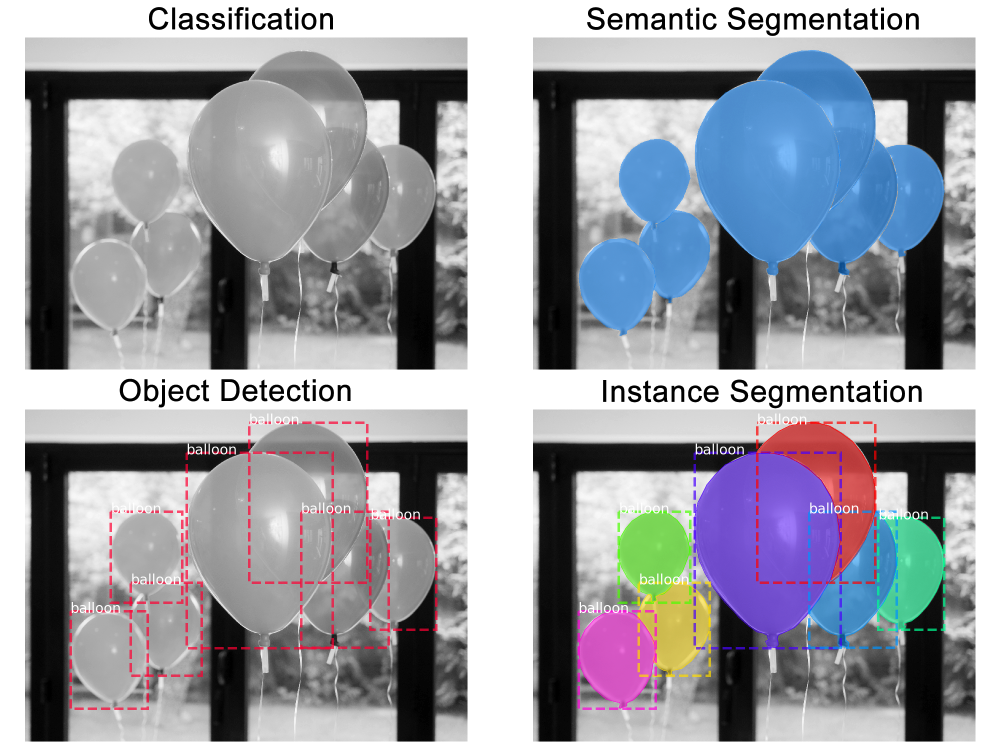
\includegraphics[scale=0.23]{figuras/image-segmentation-types}
    \source{\cite{MediumInstanceSegmentation2019}}
  \end{figure}
\end{frame}

\begin{frame}{Segmentação interativa}
  \begin{figure}\label{fig:interactive--segmentation}
    \centering
    \caption{Ilustração de segmentação interativa, rotulações em azul  e
      vermelho.\\ Na imagem à direita, após segmentação o fundo foi removido.}
    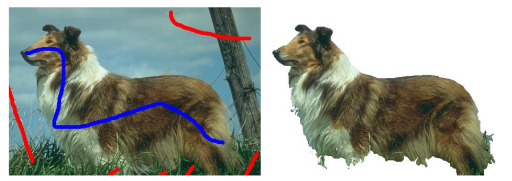
\includegraphics[scale=0.6]{figuras/interactive-segmentation-2008}
    \source{\cite{duchenne2008segmentation}}
  \end{figure}
\end{frame}

%% ---------------------------------------------------------------------------
\subsection{Aprendizado de máquina}

\begin{frame}{Aprendizado de máquina}
  Em~\cite{samuel1959some}, aprendizado de maquina é definido como:

  \begin{block}{Definição} Campo de estudo que dá aos computadores a
    habilidade de aprender sem serem explicitamente programados.
  \end{block}

  \pause{}

  \begin{figure}\label{fig:samuel}
    \centering
    \caption{
      Arthur Samuel, 1956, apresenta sua criação ao público na
      TV, uma inteligência artificial capaz de jogar damas no
      computador IBM 701.
    }
    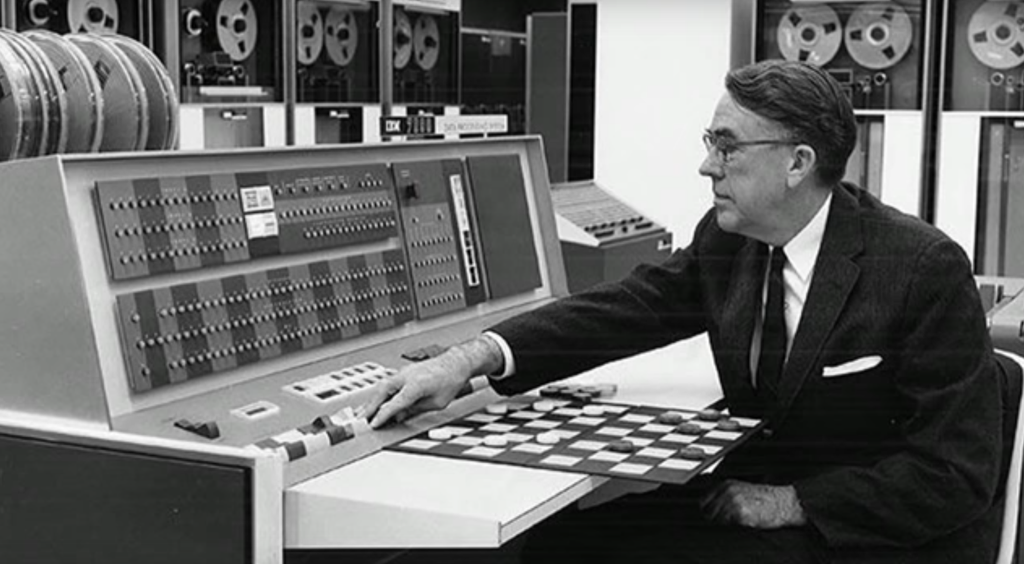
\includegraphics[scale=0.18]{figuras/samuel}
    \source{\cite{press2021machine}}
  \end{figure}
\end{frame}

\begin{frame}{Aprendizado semi-supervisionado}
  \begin{figure}\label{fig:ilustracao-aprendizado-semi-supervisionado}
    \centering
    \caption{
      O aprendizado semi-supervisionado tem como principal
característica \\ a utilização de dados rotulados e não rotulados na base
de treinamento.
}
    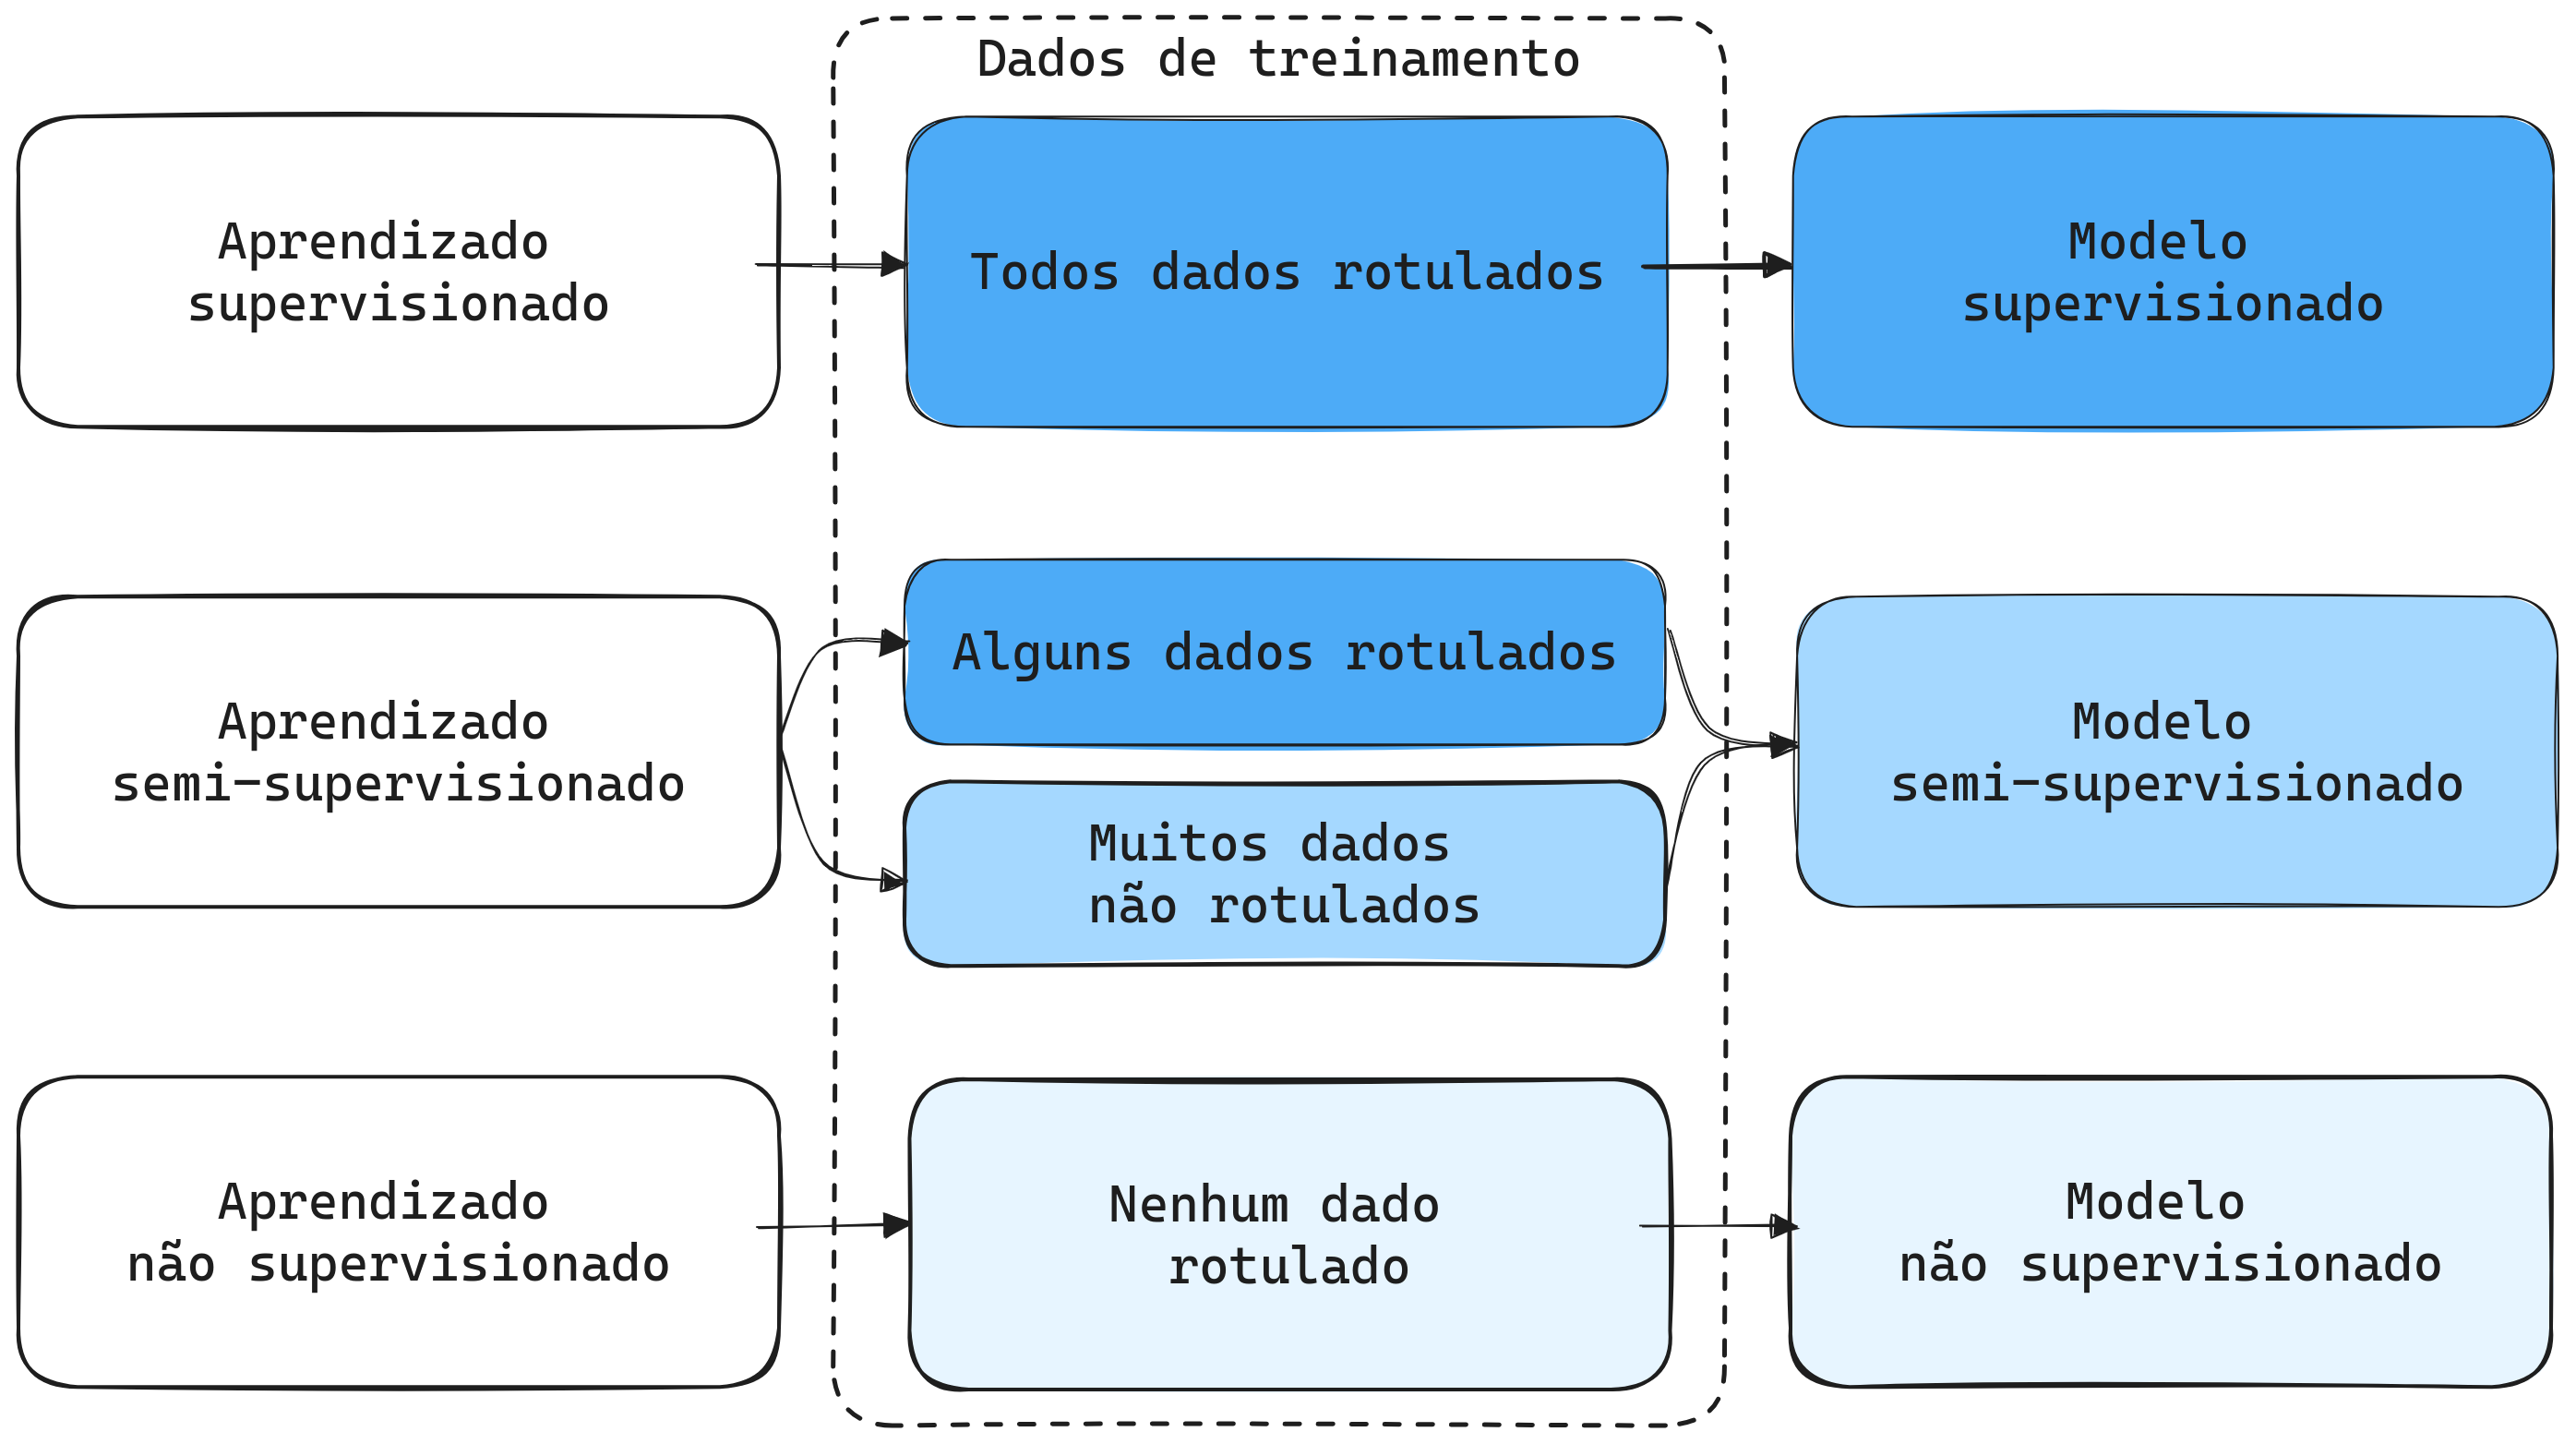
\includegraphics[scale=0.1]{figuras/ilustracao-aprendizado-semi-supervisionado}
    \source{\fonteautor}
  \end{figure}
\end{frame}


\begin{frame}{Aprendizado semi-supervisionado}
  \begin{block}{Dados de treinamento}
    Dado um conjunto de dados de treinamento $ \mathbf{X} =
    \{\vec{x_1}, \vec{x_2}, \ldots, \vec{x_n}\} $, tal que $ \vec{x_n} \in \mathbb{R}^d $,
    apenas um subconjunto $ \vec{Y} = \{y_1, y_2, \ldots , y_m\} $,
    em que $ (m < n) $, tem rótulos correspondentes.
  \end{block}

  \pause{}

  \begin{block}{Objetivo}
    O objetivo do aprendizado semi-supervisionado é usar tanto o
conjunto de dados rotulado quanto o não rotulado para aprender a
função $ f: \mathbf{X} \rightarrow \vec{Y} $ que pode prever o rótulo $ y $ para
um novo exemplo $ \vec{x} $.
  \end{block}
\end{frame}


\subsection{Aprendizado indutivo vs aprendizado transdutivo}

\begin{frame}{Aprendizado indutivo vs aprendizado transdutivo}
  \begin{figure}\label{fig:induction-vs-transudciton-cropped}
    \centering
    \caption{
      No aprendizado indutivo, como em redes neurais, uma função de
inferência é estimada durante o treinamento. Enquanto isso,
no aprendizado transdutivo a inferência de novos pontos é realizado sem a
necessidade de estimar essa função.
}
    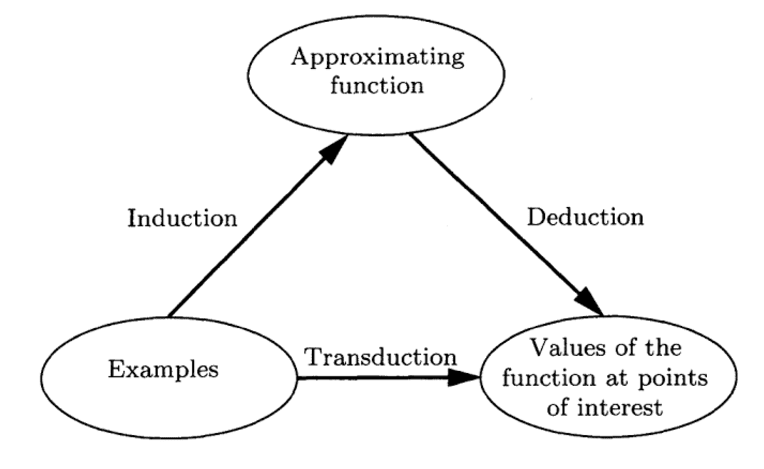
\includegraphics[scale=0.42]{figuras/induction_vs_transduction_cropped}
    \source{\cite{vapnik1995}}
  \end{figure}
\end{frame}

\begin{frame}{Aprendizado indutivo vs aprendizado transdutivo}
  \begin{figure}\label{fig:transductive-vs-inductive}
    \centering
    \caption{ Uma ilustração de aprendizado indutivo e aprendizado
      transdutivo.  }
    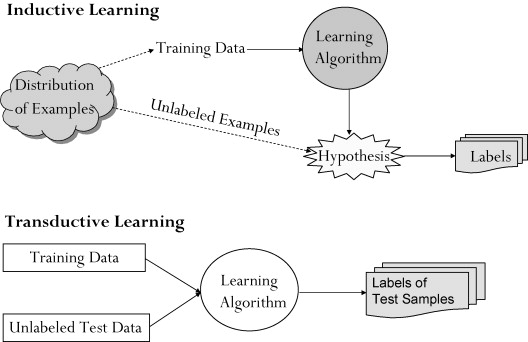
\includegraphics[scale=0.75]{figuras/transductive-vs-inductive}
    \source{\cite{vapnik1995}}
  \end{figure}
\end{frame}

\begin{frame}{Aprendizado indutivo vs aprendizado transdutivo}
  \begin{exampleblock}{Analogia}
    O aprendizado indutivo pode ser considerado um sistema de educação que
alcança um entendimento generalizado, enquanto o aprendizado
transdutivo é um sistema de educação focado na realização de provas.
  \end{exampleblock}
\end{frame}

\subsection{Objetivos}
\begin{frame}{Objetivos}
  \begin{alertblock}{Objetivo Geral}
    Desenvolver uma nova técnica de segmentação de imagens
    semi-supervisionada que possa ser equiparável ao estado-da-arte, com
    foco em \textbf{segmentação interativa}.
  \end{alertblock}
  \pause{}
  \begin{itemize}[<+->]
  \item Explorar técnicas de redes complexas e dinâmicas coletivas sobre
    o problema de segmentação de imagens;
  \item Aplicar em casos variados de segmentação de imagens, como
    objetos comuns, carros, pessoas, etc.;
  \item Avaliar o impacto da segmentação por superpixel na segmentação final;
  \end{itemize}

\end{frame}


%% -----------------------------------------------------------------------------------
%% ----- FUNDAMENTAÇÃO TEÓRICA ---------
%% ------------------------------------------------------------------------------------
\section{Fundamentação Teórica}
\subsection{Superpixels}
\subsection{Redes complexas}
\subsection{Extração de características}
\subsection{Dinâmicas coletivas}
\subsection{EGSIS}

%% -----------------------------------------------------------------------------------
%% ---------- METODOLOGIA ------------------------------------
%% -------------------------------------------------------------------------------------
\section{Metodologia}

%%
\subsection{Dataset GrabCut}

\subsection{Métricas de avaliação}


\section{Resultados}

\subsection{Variação na quantidade de superpixels}
\subsection{Resultados qualitativos}
\subsection{Resultados quantitativos}

\section{Conclusão}
\begin{frame}{Principais conclusões}
  \begin{enumerate}[<+->]

  \item Desenvolvimento de um novo algoritmo chamado EGSIS que permite
    a resolução de problemas de segmentação interativa de imagens.

  \item O algoritmo EGSIS apresentou uma \textbf{eficácia equiparável}
    aos métodos estado-da-arte baseados em grafos para segmentação
    interativa de imagens.

  \item A qualidade da segmentação final é altamente dependente da
    qualidade da pré-segmentação com superpixels.

  \item Melhores resultados foram alcançados com um \textbf{maior número de
    superpixels}, mas isso também aumentou o tempo de execução do
    algoritmo.

  \item O algoritmo possui várias partes móveis e trocáveis, permitindo a
    evolução de técnicas para melhorar a qualidade de segmentação final.

  \end{enumerate}
\end{frame}

\subsection{Limitações e desafios}
\begin{frame}{Limitações e desafios}
  \begin{enumerate}[<+->]
  \item A busca por trabalhos de referência com a palavra-chave
    semi-supervisionado foi desafiadora, mas a mudança para
    \textbf{segmentação transdutiva e interativa} permitiu encontrar trabalhos
    mais relevantes.

  \item A falta de datasets para segmentação interativa com anotação
    parcial inicial limitou a exploração e comparação com outros
    datasets e técnicas, restringindo o trabalho ao dataset GrabCut.

  \item O algoritmo EGSIS permite segmentação interativa
    multi-classes, mas a dificuldade em encontrar datasets públicos com rotulações
    parciais restringiu o avanço desta linha de pesquisa.

  \item Há espaço para crescimento na pesquisa de algoritmos de
    segmentação interativa multi-classes. Um novo conjunto de dados para
    benchmark seria uma contribuição relevante.

  \end{enumerate}
\end{frame}


\subsection{Trabalhos futuros}
\begin{frame}{Trabalhos futuros}
  \begin{enumerate}[<+->]
  \item A pesquisa sobre algoritmos transdutivos de segmentação de
imagens ainda está em evolução, mas com menos volume que as técnicas
indutivas.

  \item Métodos de superpixel, extração de características, construção
da rede complexa e dinâmica coletiva são partes móveis que podem ser
refinadas.

  \item Extração de características de imagens: este trabalho
limitou-se à matrizes de co-ocorrências e filtros de Gabor. Trabalhos
futuros podem explorar \textbf{técnicas estado-da-arte de extração de
características}.

\item \textbf{Minimização do número de cliques de anotação}: estudos recentes \cite{chen2022focalclick}
  buscam técnicas que minimizem o número de cliques de anotação
  necessários para alcançar segmentações de boa qualidade.


  \end{enumerate}
\end{frame}


%% ---------------------------------------------------------------------------
% Slides de referência
\begin{frame}[allowframebreaks]
  \frametitle{Referências}
  % Inserting the references file
  \bibliography{3-pos-textuais/referencias.bib}
  %\printbibliography{}
\end{frame}

%% ---------------------------------------------------------------------------
% Slide final com agradecimento e contato
\begin{frame}{}
    \centering
    \huge{\textbf{\example{Obrigado pela atenção!}}}

    \vspace{1cm}

    \Large{\textbf{Contato:}}
    \newline
    \vspace*{0.5cm}
    \large{\email{manoel.machado@alu.ufc.br}}
\end{frame}

\end{document}
